\documentclass[twocolumn]{article}

\usepackage{graphicx}
\usepackage{biblatex}
\usepackage[spacing, tracking, kerning]{microtype}
\usepackage{fullpage}
\usepackage{titlesec}
\usepackage{float}
\usepackage{color}
\usepackage[usenames,dvipsnames,svgnames,table]{xcolor}
\usepackage{placeins}
\usepackage{dblfloatfix}
\usepackage[bottom]{footmisc}
\usepackage{amsfonts}
\newcommand{\tY}{\checkmark}
\newcommand{\tN}{$\times$}

\bibliography{refs}

\graphicspath{{./images/}}

\title{\bfseries Identifying Compiler Options to Minimize Energy Consumption for Embedded Platforms}
\author{James Pallister, Simon Hollis, Jeremy Bennett}

\titleformat{\section}{\Large\bfseries\centering}{}{0em}{}
\titleformat{\subsection}{\normalsize\bfseries}{}{0em}{}

\newcommand{\superscript}[1]{\ensuremath{^{\textrm{#1}}}}
\newcommand{\todo}[1]{\textbf{\textcolor{red}{#1}}}

\let\oldcite\cite
\renewcommand{\cite}[1]{\textsuperscript{\oldcite{#1}}}

\begin{document}
\maketitle

\begin{table*}[!hbt]
	\begin{tabular}{l l l l l}
		\textbf{Board name} & \textbf{Processor} & \textbf{RAM} & \textbf{Speed} & \textbf{Extra} \\
		\hline
		STM32F0DISCOVERY	& ARM Cortex-M0 		& 8KB		& 48 MHz		  & 64KB Flash\\
		STM32VLDISCOVERY	& ARM Cortex-M3 		& 8KB		& 24 MHz		  & 128KB Flash\\
		BeagleBone			& ARM Cortex-A8 		& 256MB		& 500 MHz		  & VFP/NEON, superscalar\\
		EMEK3				& Adapteva E16 			& 32KB/core & 400 MHz		  & FPU, superscalar, 16 core NoC\\
		XK1					& XMOS L1 				& 64KB		& 100 MHz 		& 4$\times$100MHz hardware threads \\
	\end{tabular}
	\caption{The platforms explored in this paper along with some relevant details.}
	\label{Table:Platforms}
\end{table*}

\section*{Abstract}

\textit{
Abstract astract abtrct absrct astrct abstract stract bstract
astract abtrct absrct astrct abstract bstract
astract abtrct absrct astrct stract bstract
astract abtrct absrct astrct stract bstract
astract abtrct absrct astrct abstract bstract
astractastrct abstract stract bstract
astract abtrct absrct astrct abstract bstract
astract abtrct absrct astrct stract bstract
astract abtrct absrct astrct abstract bstract
astractastrct abstract stract bstract
astract abtrct absrct astrct abstract bstract
astract abtrct absrct astrct stract bstract
astractastrct abstract stract bstract
astract abtrct absrct astrct abstract stract bstract
}

\section*{Introduction}


% Talk about energy consumption in general
% energy consumption important
% many hardware features and optimizations (clock gating) to lower power consumption
% but cant be considered independently, software must be considered too, as it controls the hardware
Energy consumption is rapidly becoming one of the most important design constraints when writing software for embedded platforms. In the hardware space there have been many features such as clock gates to reduce the power consumption of electronic devices. However, due to the software running on top of the hardware platform, the combination of software and hardware must be taken together when exploring energy usage. \todo{as has been done in...}

% talk about embedded platforms
% lots of different architectures
% each has different energy consumption characteristics
%talk about power, aswell.
%less spikey power consumption,
%less overall power consumption = less bulky power supplies
Optimizing for low energy consumption is particularly important for embedded systems, where battery life is affected by the efficiency of the software. In these systems the processor is but one of the components consuming energy previous studies have established that the processor takes between 20\% and 40\% of the overall system power \todo{Find a reference for this? is this true?} For the embedded space, power consumption is also an issue. A lower power draw results in small circuitry for the power supply\todo{(REF)}.

%GCC Talk compiler optimisations affecting performance.
%Many people think that this has been done, but no extensive data gathered on.
%Mention iterative compilation paper: only looked at 2 optimisations for 3 limited test cases. Want to know if faster program=less energy.
% not many studies with real hardware measurements
Compiler optimizations have the potential for energy savings with no changes to existing applications - just tweaking the compiler's parameters can have a large effect on the performance. This relationship is complex, with the program, processor architecture and specific compiler options interacting together. Furthermore, different optimization passes interact with each other meaning that an option cannot be tested in isolation \todo{(PREVIOUS WORK HAS SHOWN THIS. TODO: FIND SOME)}. For example, inlining a function may mean that more effective common expression elimination can be performed, reducing the instruction count more than either option individually.

% hardware
All the energy measurements in this paper are taken using physical measurement circuitry attached to the processors. This avoids the use of models which could be inaccurate, or modelling synthetic processors with no real world counterpart. By using commonly available platforms and processors along with some more novel architectures, the results are applicable in general while still providing insight into how different types of architectures perform. There are five platforms examined in this paper, shown in Table~\ref{Table:Platforms}.

In this paper several experiments exploring the optimization passes enabled at different optimization levels are conducted. Each experiment uses the fractional factorial design method to deal with the interactions between optimizations.


%Talk about how different benchmarks are needed, taken from contempory, chosen to be implementable,
%short paragraph, quick justification.
A set of benchmarks has been derived from contemporary suites, chosen to be implementable on the target platforms. This set of 10 benchmarks (shown in Table~\ref{Table:Benchmarks}) covers real world and synthetic applications coving different aspects of the target platform. The benchmarks cover combinations of the following criteria:
\begin{itemize}
	\setlength{\itemsep}{0em}
	% \setlength{\parskip}{1pt}
	\vspace{-1mm}
	\item \textbf{Integer pipeline intensity.} The frequency at which integer arithmetic instructions occur.
	\item \textbf{Floating point intensity.} The frequency of floating point operations.
	\item \textbf{Memory intensity.} This is whether the program requires a large amount of memory bandwidth or not.
	\item \textbf{Branch frequency.} This metric describes how often the code branches.
\end{itemize}

These benchmarks were constructed to run on the `bare metal' - no host OS needed. This reduces the possibility that the benchmark will be pre-empted by an operating system performing a background task.

\begin{table}
	\centering
	\begin{tabular}{l c l}
	\textbf{Name}			& \textbf{Source} 	& \textbf{Category} \\
	\hline
	2d fir					& WCET 		& automotive, consumer	\\
	blowfish				& MiBench 	& security	\\
	crc32					& MiBench 	& network, telecomm	\\
	cubic solver			& MiBench 	& automotive	\\
	dijkstra				& MiBench 	& network	\\
	fdct					& WCET 		& consumer	\\
	float matmult			& WCET 		& automotive, consumer	\\
	int matmult				& WCET	 	& automotive	\\
	rjindael				& MiBench 	& security	\\
	sha						& MiBench 	& network, security	\\
	\end{tabular}
\caption{Benchmarks selected, and the categories they fit into. These are selected from MiBench\cite{MiBench} and the Worst Case Execution Time (WCET)\cite{WCET} suites.}
\label{Table:Benchmarks}
\end{table}

% Briefly discuss what we do
% Using fractional factorial design
% Using a fractional factorial design the individual optimizations comprising each optimization level in GCC are analysed for their main and two-way interactions.
% This paper extensively evaluates possible optimizations available in GCC.

This paper covers the design and results of the experiment. First, previous work in this space is discussed, along with the novel contribution this paper makes. After this, the approach and a brief discussion of fractional factorial design is listed. Then, the experiments performed presented with results. Finally, the results are evaluated and the conclusions drawn are presented.

\section*{Previous work}

% Mention not much previous work. Lots of work done on performance, and mostly assumed to carry over. Not much done with real hardware
To date there has been very little work extensively exploring the effect that different compilers optimizations have on energy consumption. Most studies focus on only a few optimizations in isolation, and few consider multiple platforms with with different architectural features.

% TODO talk about wattch, physical measurements better? looking for interesting results, as wattch is just an abstraction they may be missed. only used in one configuration mostly, energy could be very dependent on pipeline.
Many papers \todo{(TODO such as ..MORE)} discussing energy choose to use the Wattch simulator\cite{Wattch}. The accuracy of Wattch is established at being within 10\% of industry layout-level power tool. However, when simulating a program with a single optimization pass turned on, the effects may be small enough to be mistaken for error when using the Wattch framework. Additionally, energy consumption effects may not have been modelled by the simulator, potentially missing interesting effects. \todo{(OTHER SIMULATORS)}

% Talk a lot about iterative compilation for energy paper. lack of benchmarks, only looks at loop unrolling and tilesize (todo check).
%The only tests they did were matrix multiplication, vector by matrix multiplication (and one more).
%Also only one architecture (wattch).
%The energy consumption might be very dependant on the architecture and way the pipeline is structured, so their results may not be applicable to other platforms.
Iterative compilation has been examined as a possibility for choosing optimizations that reduce power by Gheorghita, Corporaal and Basten\cite{IterativeCompilationForEnergy}. In this paper, the effect of different loop unrolling and loop tiling parameters on energy consumption was examined for three benchmarks --- all matrix-based benchmarks. The energy consumption was estimated using the Wattch simulator as opposed to taking hardware measurements. They came to the conclusion that iterative compilation was an effective method of decreasing energy consumption as well as improving performance.

%However iterative compilation does not account for interactions between the optimization passes which could potentially have N! combinations to explore.

\todo{TODO MILEPOST}

% performance==energy, only tested the overall optimization levels O1-O4 and 4 individual optimizations, simulated with wattch - inherits all the inaccuracies that wattch might have. the 4 individual optimizations are only applied individual, no exploration of the interactions between them is attempted. ar
The topic of performance and energy being highly correlated is addressed in `Is Compiling for Performance == Compiling for Power?'\cite{CompilingForPerformancePower}. The paper explored several different overall optimization levels, as well as four specific optimizations, also using the Wattch simulator to gather energy results. However the specific optimizations were all applied individually on top of \texttt{-O1}, without exploring any possible interactions between the optimizations. The main conclusion drawn from this study was that most optimizations reduce the number of instructions executed, hence reducing energy consumption and execution time simultaneously.

% compilation techniques for low energy
% identified that the following could be used by compilers to reduce energy:
% 	reordering to reduce switching
% 	reducing memory accesses
% 	improving cache hits
% 	reduce switching on address lines
% 	improve page hits
An analysis of what a compiler can do to optimize for energy was carried out by Tiwari, Malik and Wolfe\cite{CompilationTechniquesForLowEnergy}. In this, they identified several ways possible techniques that compilers could use to reduce the energy consumption of programs:
\begin{itemize}
	\setlength{\itemsep}{0em}
	\vspace{-1mm}

	\item Reorder instructions to reduce switching.
	\item Reduce switching on address lines.
	\item Reduce memory accesses.
	\item Improve cache hits.
	\item Improve page hits.
\end{itemize}

It is expected that optimizations that cover some of these points will have an effect on energy. The last three will also normally increase performance as well as reduce energy.

% what can the poor compiler do - most measurements on gatelevel sim. only one platform
Another paper addresses the types of effects optimizations can have on performance and energy\cite{WhatCanAPoorCompilerDo}. This paper took a both hardware measurements and used a gate-level simulation to derive the results,  separating the optimizations into three classes:
\begin{itemize}
	\setlength{\itemsep}{0em}
	\vspace{-1mm}
	\item Reduction in energy consumption due to increase in performance. These optimizations reduce the number of cycles or instructions needed to complete the application and thus less overall work is done because.
	\item Optimizations that reduce energy while not improving the performance. Scheduling instructions to reduce switching often falls into this category.
	\item Optimizations that increase energy consumption or performance. These would typically be bad optimizations to choose.
\end{itemize}

\textcolor{blue}{One of our contributions is to show a fourth category exists: optimizations that increase energy consumption while increasing performance. This is in opposition to the second category listed above.}

Architectural modifications to embedded processors have been proposed as a way to save energy. Guan and Fei investigated partitioning the register file\cite{RegisterFilePartitioning} into hot and cold regions to save energy. Registers were reallocated after compilation to enhance the benefit of this technique. Another modification possible is changing the instruction encoding to minimize switching between consecutive instructions. This was examined in `Low-Power Instruction Encoding Techniques'\cite{LowPowerInstructionEncodings}.

\todo{TALK ABOUT NOVEL COMPILER OPTIMIZATIONS TO REDUCE ENERGY - reduce switching on address lines, register renaming, scheduling cost based on switching.}


\section*{Approach}

We believe that all these studies are limited and bear insufficient resemblance to modern embedded systems. Furthermore, iterative compilation can leave holes of potential combinations of optimizations unexplored. This could lead to the most optimal configuration not being found. In this paper we present another technique for testing the effectiveness of large numbers of compile optimization flags and their impact on energy consumption and run-times. The technique is based on the concept of fractional factorial designs (discussed in the following section).

In this paper we explore the impact of compiler optimizations using the GCC toolchain on the architectures in Table~\ref{Table:Platforms}. We explore what flags are and are not significant.

\todo{Mention that we explore the optimizations GCC exposes as flags. Most of them grouped into O1-3}


\section*{Fractional Factorial Design}

GCC has over 150 different option that can be enabled to control optimizations. The majority of these options are binary --- the optimization pass is either enabled or disabled. To further complicate matters, an optimization path may be affect by other passes happening before it. As it is infeasible to test all possible combinations of options, a trade-off can be made. Using a fractional factorial design (FFD), adequate data can be gathered with a much reduced set of runs. This approach has been explored before in `Feedback-Directed Selection and Characterization of Compiler Optimizations'\cite{IntelPaper}, where 9 optimizations were explored in just 35 tests as opposed to the 512 required for a full factorial design.

The drawback to this approach is that the high-order interactions between options will not be discernible. Fortunately this is not usually a problem as these types of interactions are statistically rare\todo{\cite{REF sparsity of effects?}}. The degree to which this happens is specified by the FFD's resolution\cite{BoxHunter}. A resolution 5 design ensures that the main effects are not aliased with anything lower than 4th order interactions.

Using the Yates algorithm the effect for any single or combination of factors can be found from the data. This gives an average estimation for how much this factor or interaction affects the result of the experiment

% This section outlines the fractional factorial design (FFD) method used in this paper.

% Fractional Factorial design. Mention intel paper

% Quick overview of how FFD works. Introduce resolutions, mention that compiler options should possible have many highorder interactions

All FFDs used were generated by R, using the FrF2 library\cite{FrF2}.


%Result graph here for better placement
\begin{figure*}[tb!]
	\centering
	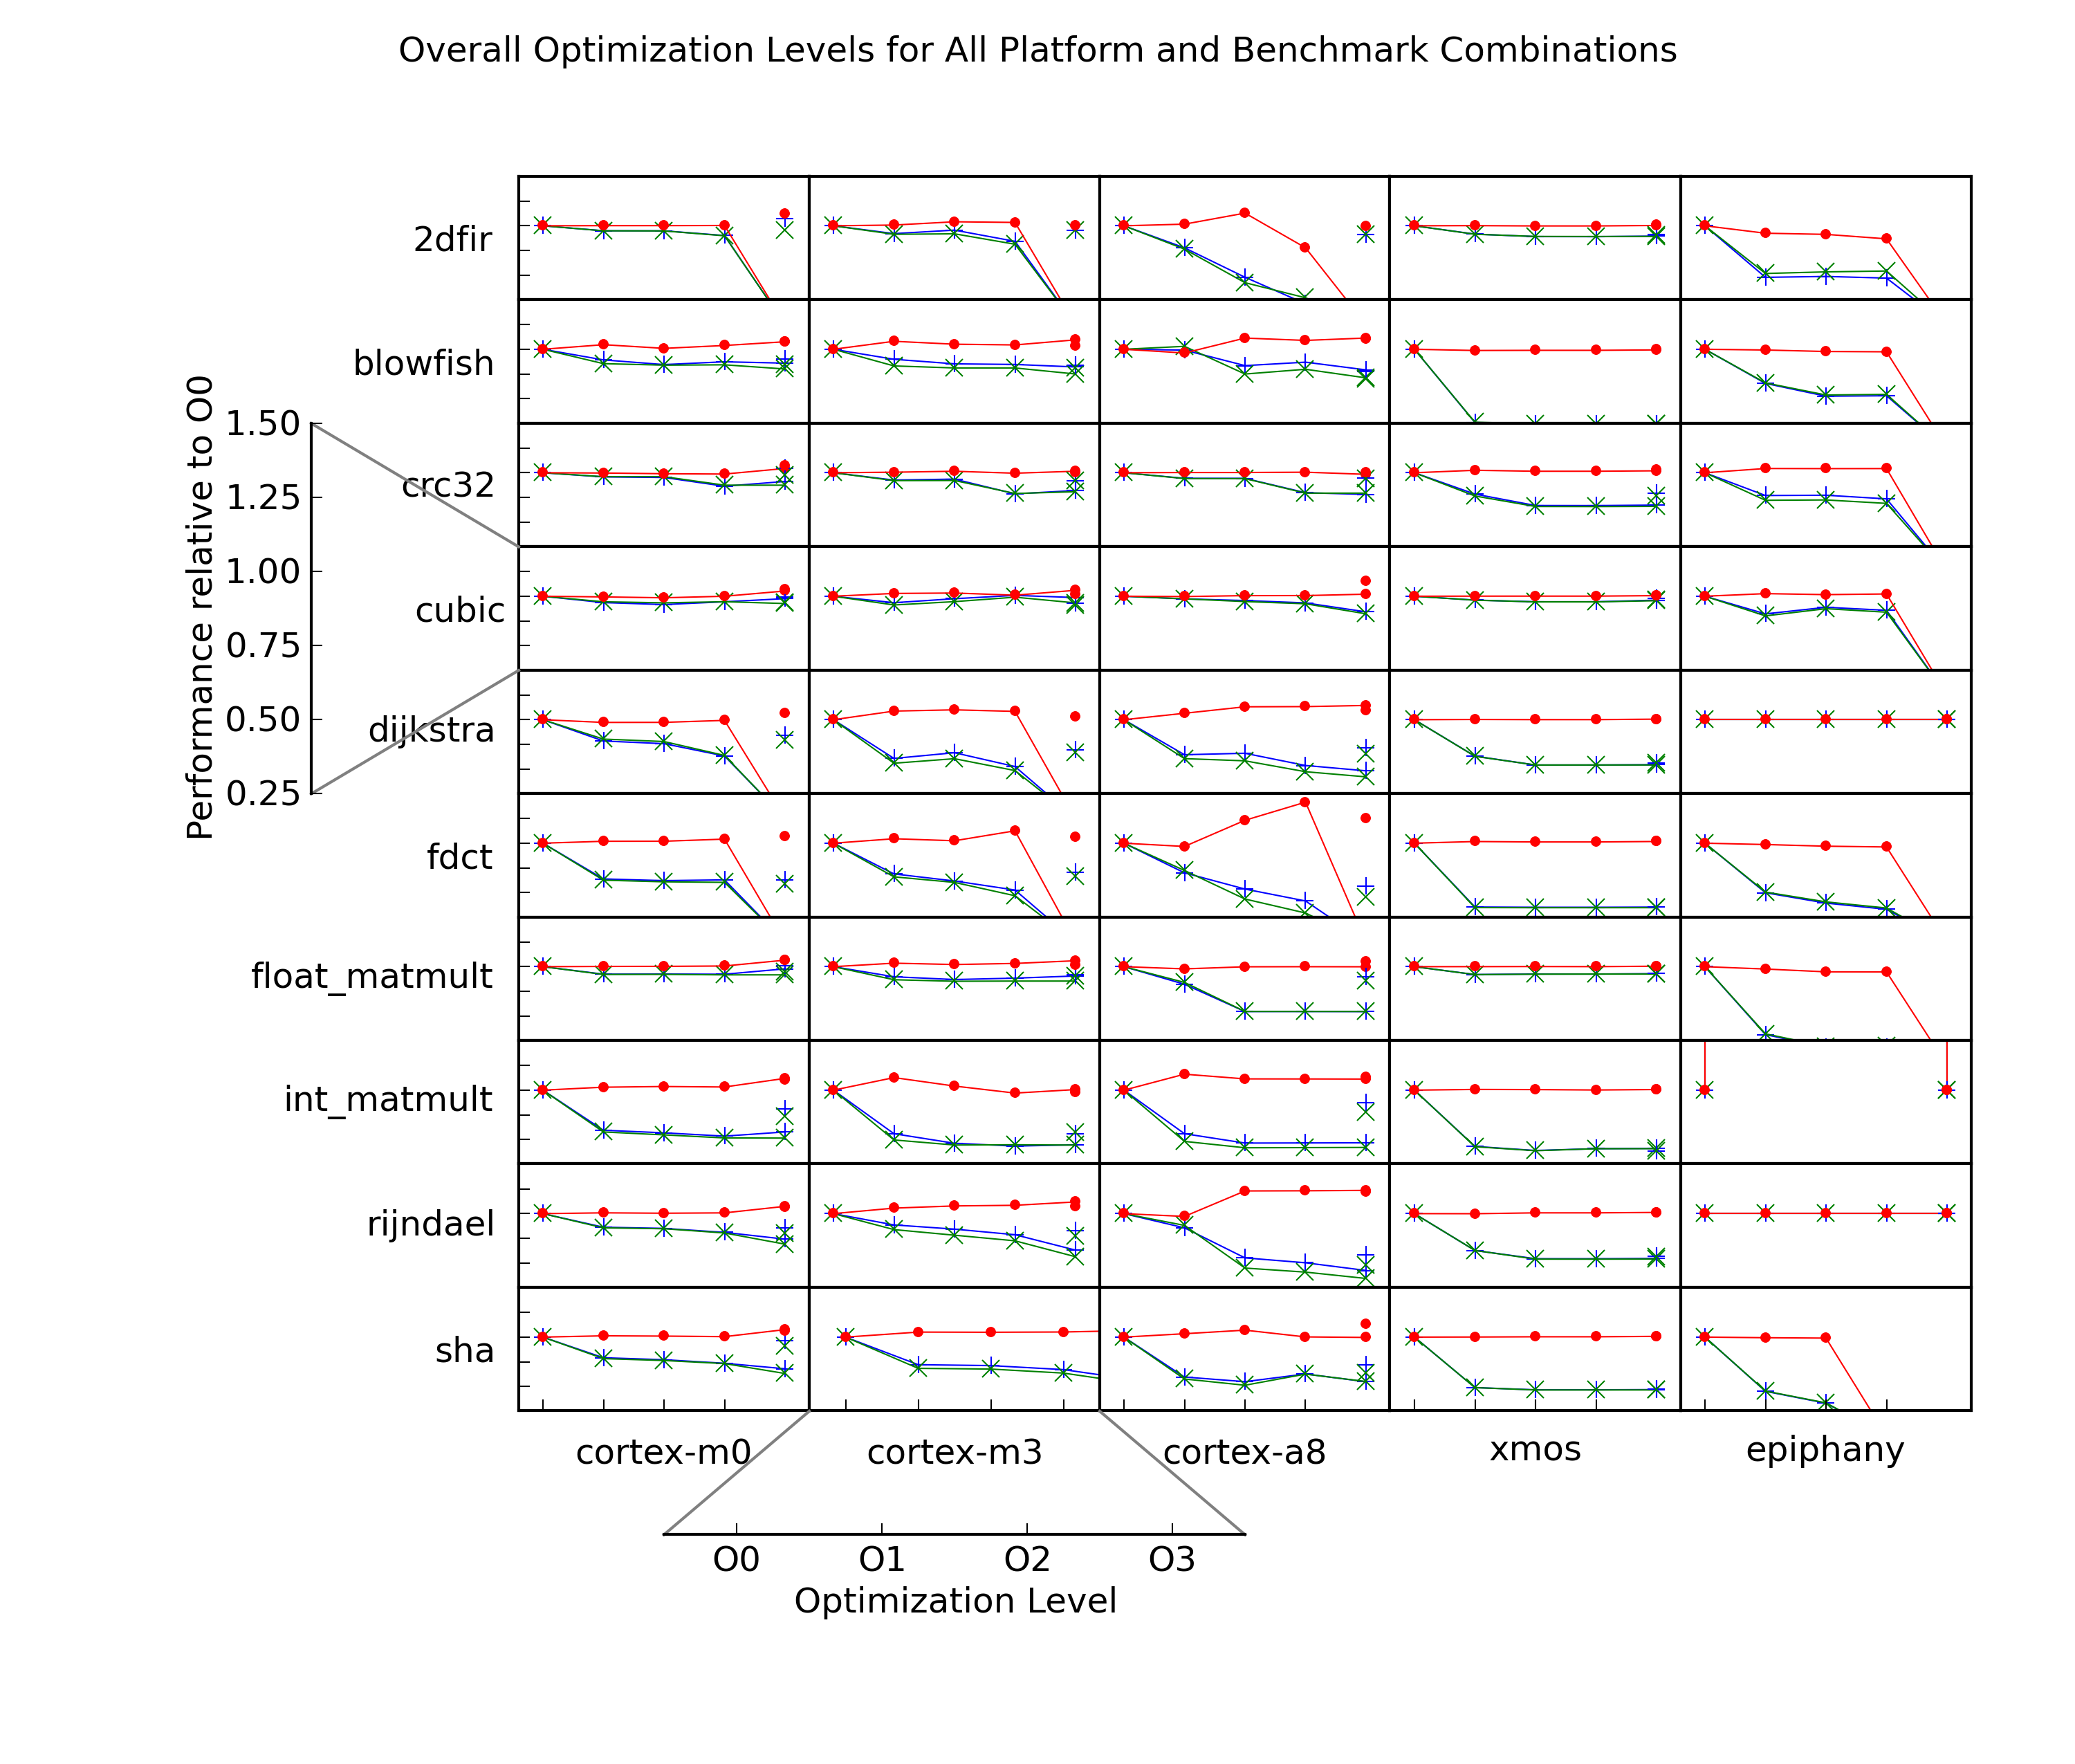
\includegraphics[width=\textwidth,clip, trim=2cm 1.5cm 0 0]{levels.png}
	\caption{Energy, Time and Power results for benchmark-platform combinations. Optimization levels \texttt{O0} to \texttt{O3}. \todo{TODO:finish}}
	\label{Fig:OverallView}
\end{figure*}

\section*{Experimental Design}

This section talks about the individual experiments that were run on the hardware. For each platform and benchmark combination the following experiments were ran.

\subsection*{First Optimization Level (O1)}

An FFD design of resolution 5 was used to evaluate GCC's 37 flags turned on by \texttt{-O1}. This consisted of 2048 different runs, allowing the main factors to be examined. If third order interactions are considered negligible, two way interactions of the flags can be resolved. The experiment aimed to identify which of the flags in this optimization level has the largest impact on energy consumption and execution time.

\subsection*{Second Optimization Level (O2)}

As with the \texttt{O1} experiment this uses a resolution 5 FFD to examine the 36 factors enabled by \texttt{-O2}. This optimization level enables more advanced optimizations, such as instruction scheduling and various peephole optimizations.

\subsection*{Third Optimization Level (O3)}

As with the previous two experiments this uses an FFD to examine the 9 factors enabled by \texttt{-O3}. This optimization level enables the most aggressive optimizations typically used, including optimizations that increase performance at the expense of code size.

% \subsection*{Incremental Tests}

% This experiment used to data generated by the \texttt{O1} tests to cumulatively turn on the flags in order of best to worst. When compared to having all the flags on those shows the effect that a small number of optimisations can have on the code.

\subsection*{Single Flag Difference}

This experiment enabled the first optimization level (\texttt{-O1}) then individually added or subtracted possible optimisation flags. The aim of this experiment was to identify if a single flag could have a significant difference on the energy consumption.

% \subsection*{Profiling}

% Using profile guided feedback the compile can make much better guesses about what the code is going to do. This allows extra optimizations to be enabled and improves to performance of some existing optimizations.

% \subsection*{Link Time Optimization}

% When the benchmark consists of multiple compilation units, the program is not optimized as a whole. This means many of the optimizations performed could be better if done at link time.

\section*{Hardware Setup}

All the measurements were taken using the INA219 power monitoring IC\cite{INA219}, which provides power, current and voltage outputs. This chip measures the voltage drop across a small shunt resistor inline with the target circuit. For all platforms this is placed after the voltage regulator, before the main processor. Each INA219 chip is connected the an XMOS controller board to record the results and transfer them to the host PC. Each platform has a GPIO line connected to the controller. This toggled when benchmarks started and ended, allowing just the intended portion of the benchmark to be measured (ignoring any extra initialization code).

The Cortex-M0 and Cortex-M3 boards both have a single measurement point, recording the power consumed by the whole microprocessor. For the BeagleBone there were three available measurement points: the Cortex-A8 core, on-chip peripherals (caches, power management) and the external SDRAM memory IC. This allows the effect of the compiler optimizations on the memory to be recorded. Adapteva's Epiphany board had two measurement points: the core power consumption and IO power consumption, whereas the XMOS board's measurement point gathered power consumption data for the core of the processor.

\todo{talk about error bounds?}
% A few paragraphs about the hardware setup.
% Talk about INA219, error bounds, analysis of error?
% Talk about hooking the inductors


\section*{Results}

\begin{figure}[tb]
	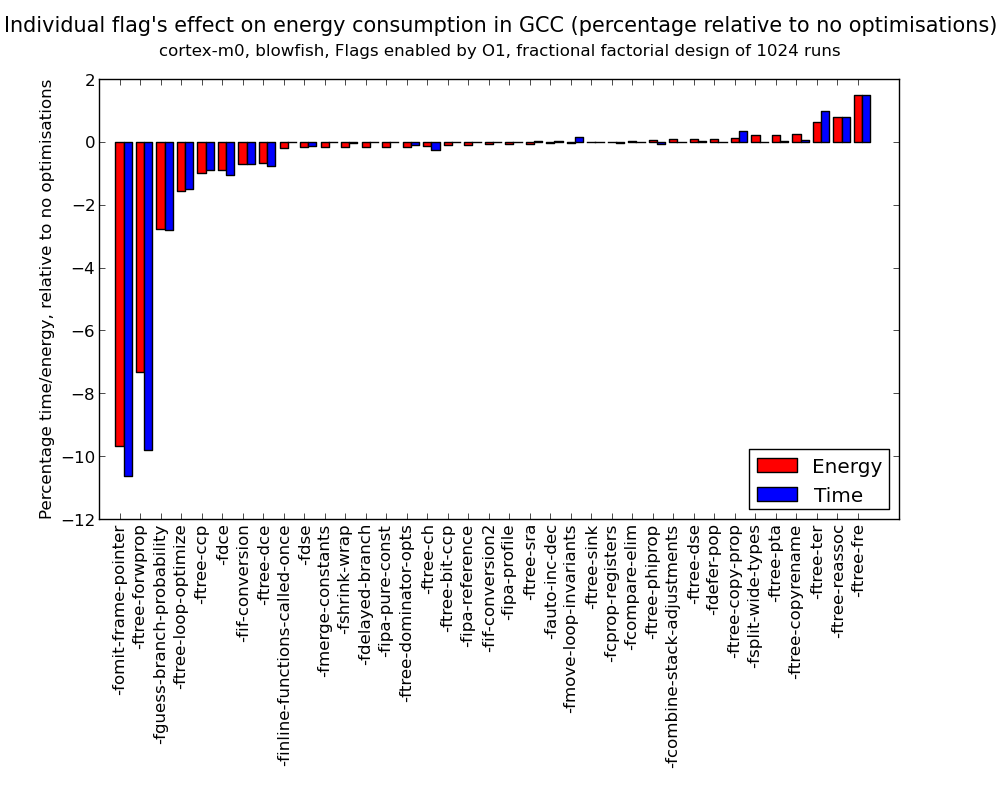
\includegraphics[width=\linewidth]{cortex-m0/O1_main_effects_blowfish.png}
	\caption{The blowfish benchmark on the Cortex-M0 platform. Individual options enabled at \texttt{O1} are listed.}
	\label{Fig:BlowfishMainEffects}
\end{figure}

\begin{figure}[tb]
	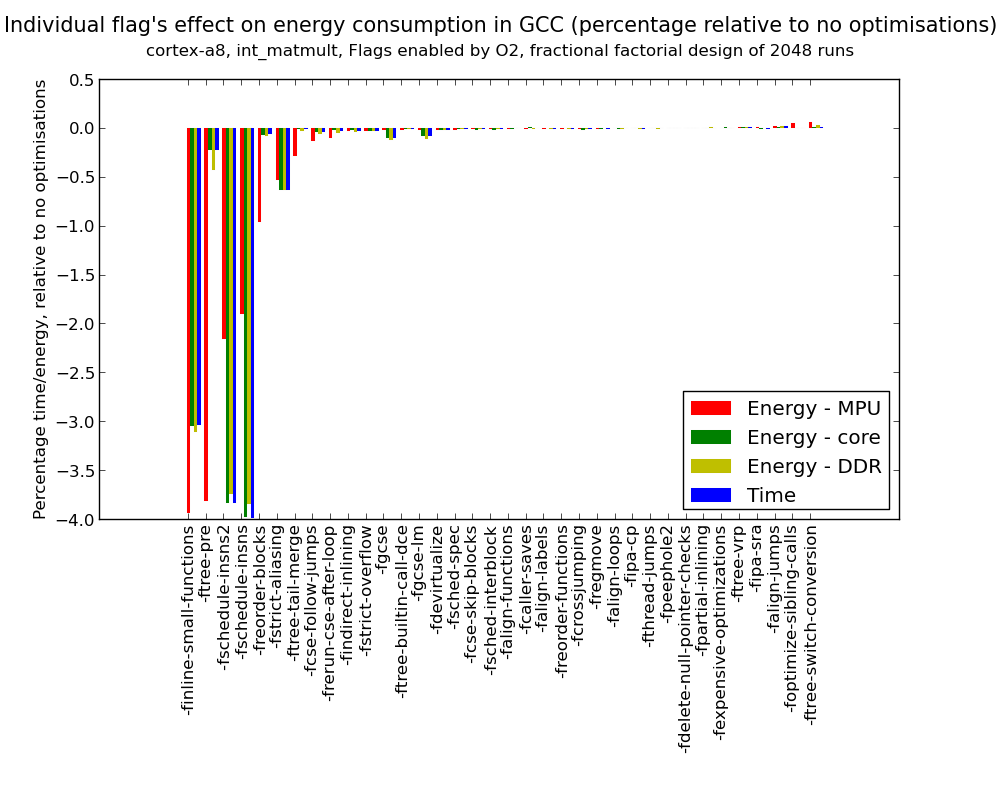
\includegraphics[width=\linewidth]{cortex-a8/O2_main_effects_int_matmult.png}
	\caption{The integer matrix multiplication benchmark on the Cortex-A8 platform. Individual options enabled at \texttt{O2} are listed.}
	\label{Fig:IntMatmultO2MainEffects}
\end{figure}

\begin{figure}[tb]
	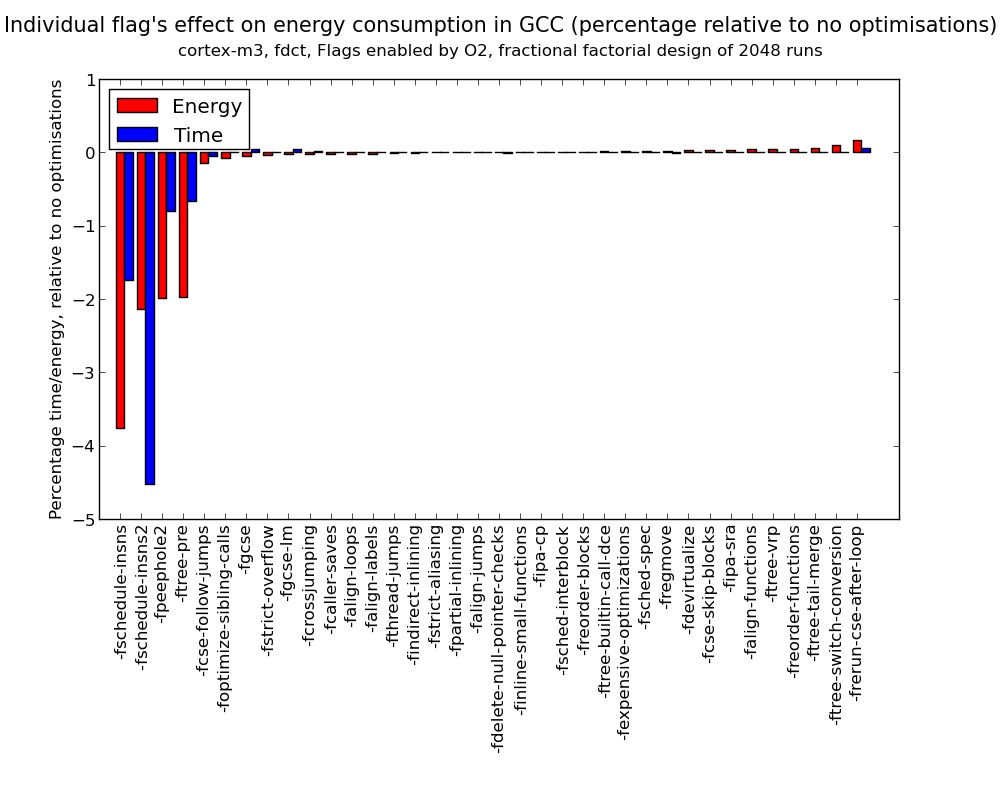
\includegraphics[width=\linewidth]{cortex-m3/O2_main_effects_fdct.png}
	\caption{The FDCT benchmark on the Cortex-M3 platform. Individual options enabled at \texttt{O2} are listed.}
	\label{Fig:FdctO2MainEffects}
\end{figure}

A high level overview of each platform and benchmark for different optimization levels is given in Figure~\ref{Fig:OverallView}. This figure shows a small line graph for each combination displaying the effect of the broad optimization levels \texttt{O1}, \texttt{O2}, \texttt{O3} on time, energy and power.

The power remains constant for most of the platforms, except for the Cortex-A8. This is likely due to the superscalar nature of the core, and high optimization levels enabling instruction scheduling for multiple instructions to be executed per cycle.

For the cubic benchmark there is a much smaller performance gain from the optimizations than with the other benchmarks. This is due to the main computational body of work being done by the precompiled libraries providing the trigonometric functions.

Another observation is that there is very little divergence between execution time and energy consumption.

\subsection*{Time and Energy}



The vast majority of optimizations showed a high correlation between decreasing the duration of the benchmark and the energy consumption decreasing. A typical example of this is shown in Figure~\ref{Fig:BlowfishMainEffects}. This shows the main effect each optimization had on the runtime and energy consumption, as calculated by FFD.

This graph also demonstrates that not all optimizations will reduce the power or energy of the program they are optimizing. Also the energy is not always modified to the same degree as performance, indicating that there are other effects than just decreasing instruction count.

In Figure~\ref{Fig:IntMatmultO2MainEffects} some of the more advanced options enabled by \texttt{O2} are explored. The compiler flag \texttt{-ftree-pre} is unusual in this case in that it causes a reduction in the energy consumption of the benchmark while not reducing the execution time significantly. This flag enables partial redundancy elimination on trees.

Figure~\ref{Fig:FdctO2MainEffects} highlights the discrepancy that can occur between execution time and energy consumption, even for very similar optimizations. The first two options listed (\texttt{-fschedule-insns} and \texttt{-fschedule-insns2}) both schedule instructions to reduce instruction stalls. However the latter option performs its scheduling pass after register allocation, where as the first performs it before. In this case scheduling before the register allocation reduces the energy consumption by much more than the execution time.

% \todo{mostly true.}
% \todo{some cases when not the case. why is this?}
% \todo{suggest in some cases, without changing performance you can reduce energy}
% \todo{talk when arent the same.}
% \todo{reasons for that}

\subsection{Individual Optimizations}

In Figure~\ref{Fig:AddsubO1Blowfish} optimizations are switch on or off, and plotted relative to the \texttt{O1} optimization level. The flags in the \texttt{O1} group are turned off for the experiment, whereas the flags for \texttt{O2} and higher are turned on. This shows that some flags decrease the energy consumption of the program when turned off individually. These can be seen at the left of the graph.

These flags in particular are interesting because when turned off they decrease the energy consumption while increasing the execution time.

These results were further investigated by exhaustively trying combinations of four optimizations that decreased energy consumption while having small effect on the execution time. The energy figures for this can be seen in Table~\ref{Table:Exhaustive}. The O1 column of this table shows the results when the options were applied on top of the \texttt{O1} optimization level. The O2 column shows the same but on top of the \texttt{O2} optimization level.

 From the O1 column this it can be seen that there are many interaction effect occurring between the options, as simply turning all of these options off does not decrease the energy (in fact it increases the consumption by 1.81\%). Furthermore, when disabled individually, \texttt{-fguess-branch-probability} and \texttt{-ftree-dominator-opts} decrease the energy by 2.49\% and 1.76\% respectively. However when both enabled, the energy consumption (relative to \texttt{O1}) is only 0.93\% less, worse than each flag individually.

Different results are seen entirely in the O2 column, with options that decreased energy consumption on top of O1 have little or the opposite effect when applied on top of O2
.

This unpredictability suggests that these options have many interdependencies that are difficult to predict upfront.

\todo{peephole optimization decreasing energy }

\begin{figure*}[tb]
	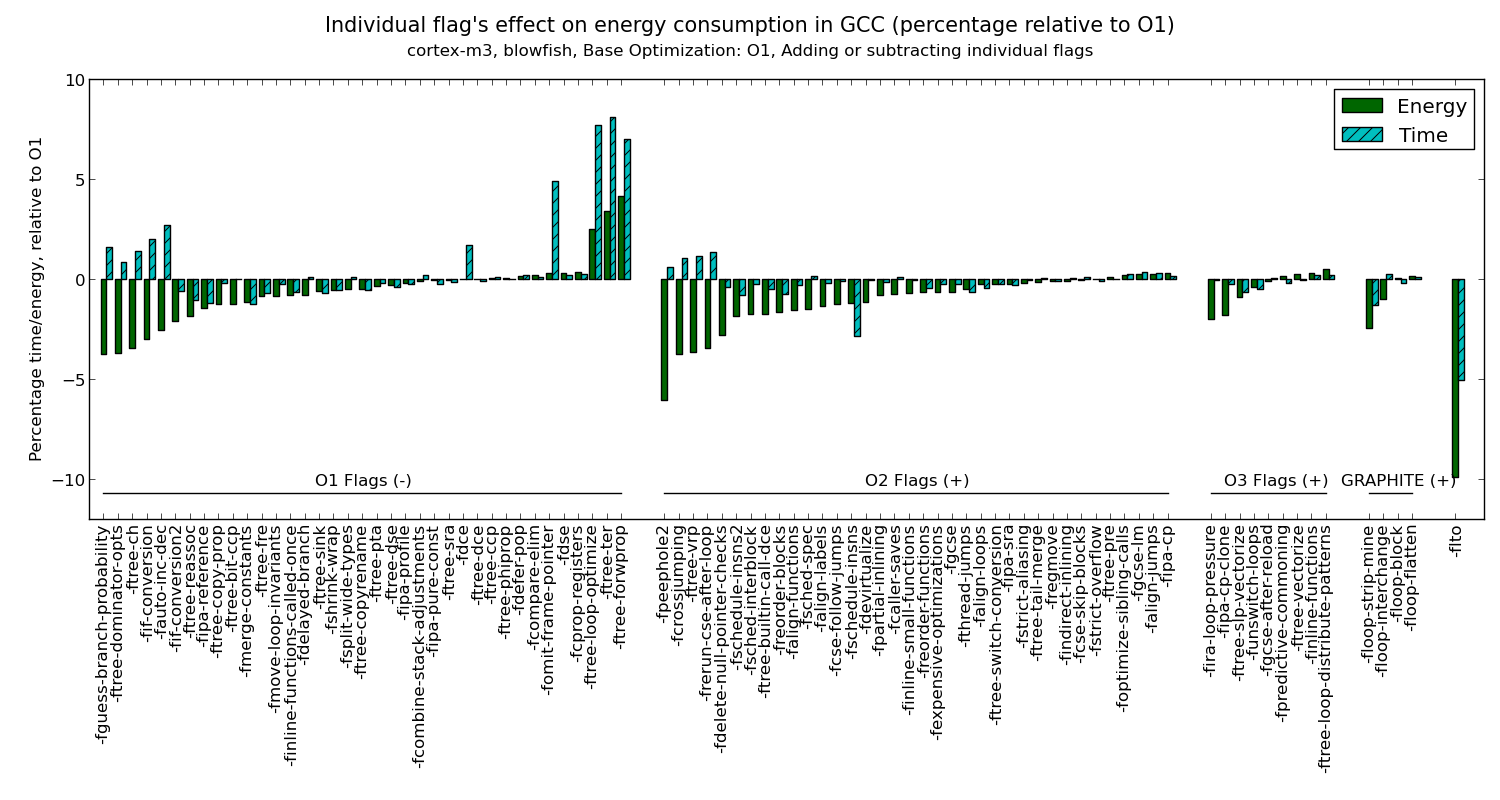
\includegraphics[width=\linewidth]{cortex-m3/O1_addsub_blowfish.png}
	\caption{The blowfish benchmark on the Cortex-M3 platform. ADDSUB Individual options enabled at \texttt{O2} are listed.}
	\label{Fig:AddsubO1Blowfish}
\end{figure*}

\begin{table}
	\centering
	\begin{tabular}{c c c c c r@{.}l c r@{.}l }
		& & & \multicolumn{3}{c}{\hspace{1.5cm}\bfseries O1} & \multicolumn{3}{c}{\hspace{1.3cm}\bfseries O2} \\
		\bfseries 1 & \bfseries 2 & \bfseries 3 & \bfseries 4 & \bfseries (mJ) 	 & \multicolumn{2}{c}{\bfseries (\%)} &
		\bfseries (mJ) 	 & \multicolumn{2}{c}{\bfseries (\%)} \\
		\hline
		\tY&\tY&\tY&\tY& 5779 & 0&00 	&  5483 &  0&00\\
		\tN&\tY&\tY&\tY& 5635 & -2&49 	&  5538 &  1&00\\
		\tY&\tN&\tY&\tY& 5677 & -1&76 	&  5480 & -0&05\\
		\tN&\tN&\tY&\tY& 5725 & -0&93 	&  5619 &  2&49\\
		\tY&\tY&\tN&\tY& 5647 & -2&28 	&  5487 &  0&09\\
		\tN&\tY&\tN&\tY& 5723 & -0&97 	&  5579 &  1&75\\
		\tY&\tN&\tN&\tY& 5611 & -2&90 	&  5481 &  -0&03\\
		\tN&\tN&\tN&\tY& 5644 & -2&33 	&  5529 &  0&85\\

		\tY&\tY&\tY&\tN& 5759 & -0&34 	&  5459 &  -0&43\\
		\tN&\tY&\tY&\tN& 5716 & -1&09 	&  5484 &  0&03\\
		\tY&\tN&\tY&\tN& 5863 & 1&45 	&  5491 &  0&15\\
		\tN&\tN&\tY&\tN& 5957 & 3&08 	&  5483 &  0&00\\
		\tY&\tY&\tN&\tN& 5889 & 1&91 	&  5472 &  -0&19\\
		\tN&\tY&\tN&\tN& 5872 & 1&61 	&  5569 &  1&57\\
		\tY&\tN&\tN&\tN& 5689 & -1&56 	&  5481 &  -0&03\\
		\tN&\tN&\tN&\tN& 5884 & 1&81 	&  5505 &  0&41\\
	\end{tabular}\\[1em]

	\begin{tabular}{l p{0.65\linewidth}}
		\bfseries Key & \bfseries Option \\
		\hline
		1 & \texttt{guess-branch-probability}  \\
		2 & \texttt{tree-dominator-opts}  \\
		3 & \texttt{tree-ch} \\
		4 & \texttt{if-conversion} \\
		Abs (mJ) & Absolute energy measurement in millijoules \\
		O1 (\%) & Percentage relative to \texttt{O1} \\
		O2 (\%) & Percentage relative to \texttt{O2} \\
	\end{tabular}
	\caption{Data and Legend when exhaustively exploring 4 options compared to \texttt{O1} and \texttt{O2}. (Cortex-M3 with blowfish benchmark).}
	\label{Table:Exhaustive}
\end{table}


% talk about what the results are briefly
% second and third order interactions

\subsection{Comparison of Platforms}

Table~\ref{Table:BestFlags} lists the single best optimization flag for each benchmark and platform combination. It can be seen that in many cases the most effective option is the same across platforms. Furthermore, only 12 \todo{(update when more results taken)} out of 82 options (the number of flags enabled by \texttt{O1}, \texttt{O2} and \texttt{O3}) appear in the table. This adds weight to the argument that many of the options have little effect on the energy consumption (and performance).

\begin{table*}
	\centering
	\begin{tabular}{l >{\ttfamily} p{0.3\linewidth} >{\ttfamily} p{0.3\linewidth} }
		\bfseries Benchmark&\rmfamily\bfseries Cortex-M0&\rmfamily\bfseries Cortex-M3\\
		\hline
		2dfir			& -fguess-branch-probability & -fpeephole2				 \\
		blowfish		& -fomit-frame-pointer 		 & -ftree-forwprop			 \\
		crc32			& -fmove-loop-invariants 	 & -fmove-loop-invariants 	 \\
		cubic			& -ftree-dominator-opts 	 & -ftree-dominator-opts  	 \\
		dijkstra		& -ftree-fre 				 & -fmove-loop-invariants	 \\
		fdct			& -ftree-forwprop 			 & -ftree-forwprop 			 \\
		float\_matmult	& -ftree-loop-optimize 		 & -ftree-loop-optimize 	 \\
		int\_matmult	& -ftree-loop-optimize 		 & -ftree-loop-optimize 	 \\
		rijndael		& N/A 						 & -fomit-frame-pointer 	 \\
		sha				& -fomit-frame-pointer 		 & -ftree-loop-optimize 	 \\
	\end{tabular} \\[1em]

	\begin{tabular}{l >{\ttfamily} p{0.3\linewidth} >{\ttfamily} p{0.3\linewidth}}
		\bfseries Benchmark& \rmfamily\bfseries Cortex-A8		& \rmfamily\bfseries Epiphany\\
		\hline
		2dfir			& -ftree-pre				& -fdce \\
		blowfish		& -fschedule-insns			& \todo{-fplace-holder} \\
		crc32			& -fmove-loop-invariants	& \todo{-fplace-holder} \\
		cubic			& -ftree-dominator-opts		& \todo{-fplace-holder} \\
		dijkstra		& -fmove-loop-invariants	& \todo{-fplace-holder} \\
		fdct			& -fschedule-insns2			& \todo{-fplace-holder} \\
		float\_matmult	& -ftree-pre				& \todo{-fplace-holder} \\
		int\_matmult	& -finline-small-functions	& \todo{-fplace-holder} \\
		rijndael		& -fschedule-insns			& \todo{-fplace-holder} \\
		sha				& -fschedule-insns2			& \todo{-fplace-holder} \\
	\end{tabular}

	\caption{Table showing the most effective option for each platform-benchmark combination. Options considered were
	optimizations enabled by \texttt{O1}, \texttt{O2} and \texttt{O3} levels.}
	\label{Table:BestFlags}
\end{table*}

\todo{count, by eye add up significant factors, how many times occur across benchmark, platform, generality - specific to benchmarks or}

\todo{point some option good or bad, cant really predict, exhaustive search}

\section*{Modelling}

Talk about how the FFD can be used to predict what flags are good

\section*{Comparison with LLVM}

Just O1, O2, O3


\section*{Evaluation}

Talk about error
 - hardware measurement
 - total amonut of energy used is correct, even if sample rate is low
 - FFD
 - cold start problem
 	only affects beaglebone, as no caches otherwise, but fits in cache anyway


Draw correlations between platforms and benchmarks.

See if there is any correlation between the `execution characteristics' of the benchmark and the flags that affect it.

Can we propose a set of options that on average performs better for the benchmarks?

Why did we get these results


\section*{Conclusion}

\section*{Future Work}

\printbibliography

\end{document}


things to discuss
  some cases where omit-frame-pointer good, some bad
  sorting algorithms interesting
  cant predict
  lots of high level stuff - majority of cases time and energy correlated
    interesting where its not, but most of the time its a very small percentage that could easily be explained away
    no large optimizations which affect energy rather than execution time
